\chapter{Análisis de los resultados}\label{sec:resultados}

En esta sección se exponen los resultados de los experimentos explicados en la Sección~\ref{sec:experimentos}. En primer lugar, en la Sección \ref{sec:hipotesis} analizamos el funcionamiento de \ac{PoFL} como mecanismo de defensa. De las debilidades detectadas en esta sección surge \ac{KFC}, cuyo rendimiento como defensa analizamos, de forma comparativa con la propuesta anterior, en la sección \ref{sec:kfc_experiments}. 

\section{Análisis de PoFL como mecanismo de defensa}\label{sec:hipotesis}

A continuación veremos el rendimiento de \ac{PoFL} tanto en el caso en el que no hay ningún atacante en la red (vea Sección \ref{sec:sin_attack_pofl}) como en los escenarios A (vea Sección \ref{sec:pofl_a}) y B (vea Sección \ref{sec:pofl_b}).

\subsection{Rendimiento sin atacantes}\label{sec:sin_attack_pofl}
Al considerar el caso de que no haya ningún atacante en la red podemos observar tanto en la Tabla \ref{tab:baseline_pofl} como en la Figura \ref{fig:pofl_no_attacks} que tanto nuestra arquitecturas de referencia como aquella basada en \ac{PoFL} obtienen un rendimiento en términos de precisión
similar en todos los conjuntos de datos. Esto nos muestra que \ac{PoFL} es una buena arquitectura para el aprendizaje y una buena alternativa a nuestras arquitecturas de referencia. Esto indica que seleccionar únicamente un modelo basándose en un criterio de eficiencia en un conjunto de validación obtiene resultados similares a los de considerar todas las actualizaciones posibles.

\begin{table*}[!ht]
\centering
\begin{tabular}{lrrrrrr}
\toprule
 & \multicolumn{3}{c}{\textit{accuracy}} & \multicolumn{3}{c}{\textit{$accuracy_{10}$}}   \\
\toprule
       & \textbf{C-S} & \textbf{PoW/S} & \textbf{PoFL} & \textbf{C-S} & \textbf{PoW/S} & \textbf{PoFL}  \\ 
\toprule
\textbf{EMNIST} & 0.9810& \textbf{0.9924}& 0.9869& 0.9805& \textbf{0.9924}& 0.9845\\  
\midrule
\textbf{Fashion MNIST}& 0.9030& \textbf{0.9033}& 0.8972& \textbf{0.9041}& 0.9040& 0.8973\\ 
\midrule
\textbf{CIFAR-10}        & \textbf{0.9688}& 0.9677& 0.9569& \textbf{0.9686}& 0.9676& 0.9564\\
\bottomrule
\end{tabular}
\caption{\textit{accuracy} y \textit{$accuracy_{10}$} comparando PoFL con las arquitecturas de referencia sin ningún atacante.}\label{tab:baseline_pofl}

\end{table*}
\begin{figure}[!ht]
\begin{subfigure}{0.49\linewidth}
  \centering
  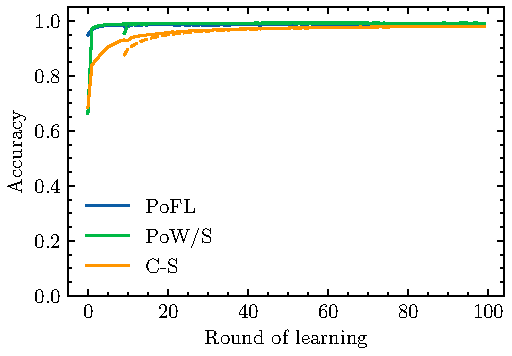
\includegraphics[width=\linewidth]{figuras/graficas/baseline_mnist_one.pdf}
  \caption{EMNIST.}
  %\label{fig:sfig1}
\end{subfigure} 
\begin{subfigure}{0.49\linewidth}
  \centering
  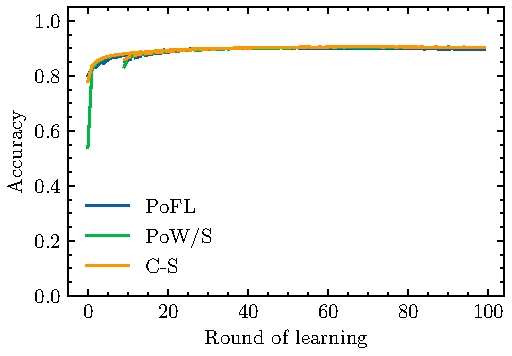
\includegraphics[width=\linewidth]{figuras/graficas/baseline_fashion_one.pdf}
  \caption{Fashion MNIST.}
  %\label{fig:sfig3}
\end{subfigure} 
\vskip\baselineskip
\centering
\begin{subfigure}{0.49\linewidth}
  \centering
  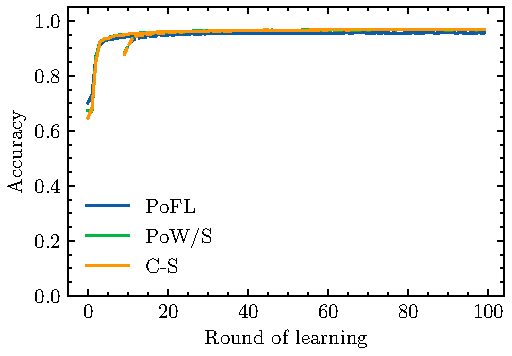
\includegraphics[width=\linewidth]{figuras/graficas/baseline_cifar_one.pdf}
  \caption{CIFAR.}
  %\label{fig:sfig2}
\end{subfigure}
\vskip\baselineskip
\caption{$accuracy$ (línea) y $accuracy_{10}$ (línea discontinua) de las tareas originales  EMNIST (a), Fashion MNIST (b) y CIFAR (c), sin ningún atacante presente.}
\label{fig:pofl_no_attacks}
\end{figure}


\newpage
\subsection{Escenario A: Un solo atacante}\label{sec:pofl_a}
En esta sección analizamos el rendimiento de \ac{PoFL} en el \textbf{escenario A}. Analizando los resultados expuestos en las Tablas \ref{tab:poflbackdoor_a} y \ref{tab:poflbyzantine_a} junto a las Figuras \ref{fig:pofl_a_backdoor} y \ref{fig:pofl_byzantine_a}, aunque se abarcan diferentes tipos de ataques, se puede observar las siguientes conclusiones comunes:

\begin{itemize}
	\item \ac{PoFL} demuestra una superioridad en rendimiento en todos los conjuntos de datos bajo ambos ataques, obteniendo la mayor precisión durante todo el proceso de entrenamiento. Además los resultados logrados por \ac{PoFL} son similares a los obtenidos para el caso donde no considerábamos atacantes, resaltando así su capacidad como mecanismo de defensa.

    \item Para nuestra tarea de \textit{backdoor}, representada en la Tabla \ref{tab:poflbackdoor_a} y Figura \ref{fig:pofl_a_backdoor}, \ac{PoFL} logra mitigar el ataque obteniendo una precisión mínima que nos sugiere la exitosa supresión de la tarea inyectada. Además, \ac{PoFL} además de mitigar el ataque consigue mantener un buen rendimiento en la tarea original, asegurando tanto la mitigación de ataques como el objetivo original. Por otra parte, nuestras arquitecturas de referencia no ofrecen ningún tipo de resistencia obteniendo una precisión casi perfecta en la tarea secundaria.

    \item Si observamos el ataque bizantino, cuyos resultados aparecen en la Tabla \ref{tab:poflbyzantine_a} y Figura \ref{fig:pofl_byzantine_a}, vemos como \ac{PoFL} vuelve a obtener los mismos resultados mientras que nuestras arquitecturas de referencia ven cómo su rendimiento es degradado presentando además múltiples perturbaciones en las medidas.
\end{itemize}

\begin{table*}[!ht]
\centering
\begin{tabular}{llrrrrrr}
\toprule
 & & \multicolumn{3}{c}{\textit{accuracy}} & \multicolumn{3}{c}{\textit{$accuracy_{10}$}}   \\
\toprule
       &          & \textbf{C-S} & \textbf{PoW/S} & \textbf{PoFL} & \textbf{C-S} & \textbf{PoW/S} & \textbf{PoFL}  \\ 
\toprule
\textbf{EMNIST} & Original & 0.9821        & 0.9793  & \textbf{0.9930}  & 0.9825        & 0.9809  & \textbf{0.9930}   \\  
       & Backdoor & 0.9999        & 0.9994  & \textbf{0.0980} & 0.9997        & 0.9996  & \textbf{0.0979}   \\  
\midrule
\textbf{Fashion}   & Original & 0.8462        & 0.8414  & \textbf{0.8961}  & 0.8416        & 0.8486  & \textbf{0.8986}  \\ 
 \textbf{MNIST}    & Backdoor & 0.9955        & 0.9969  & \textbf{0.0871}& 0.9884        & 0.9878  & \textbf{0.0989}   \\ 
\midrule
\textbf{CIFAR-10}        & Original & 0.9103        & 0.9038  & \textbf{0.9397}  & 0.9021        & 0.8762  & \textbf{0.9283}   \\ 
                & Backdoor & 0.9676        & 0.9704  & \textbf{0.1163}   & 0.9348        & 0.9736  & \textbf{0.0849}  \\ 
\bottomrule
\end{tabular}
\caption{\textit{accuracy} y \textit{$accuracy_{10}$} comparando PoFL con las arquitecturas de referencia en el \textbf{escenario A} ante un ataque de backdoor.}\label{tab:poflbackdoor_a}
\end{table*}

\begin{figure}[!ht]
\begin{subfigure}{0.49\linewidth}
  \centering
  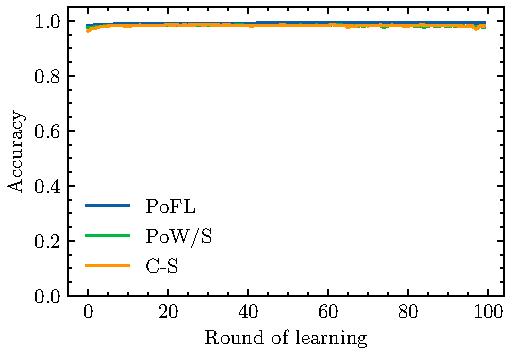
\includegraphics[width=\linewidth]{figuras/graficas/original_mnist_one.pdf}
  \caption{EMNIST (Tarea original).}
  %\label{fig:sfig1}
\end{subfigure} 
\begin{subfigure}{0.49\linewidth}
  \centering
  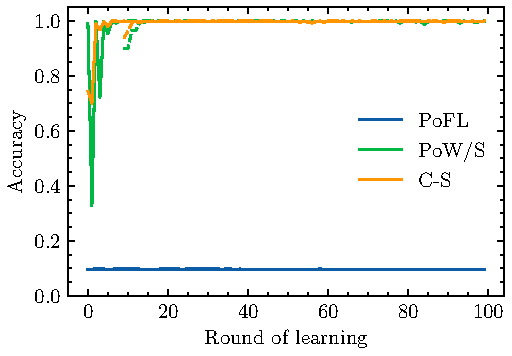
\includegraphics[width=\linewidth]{figuras/graficas/backdoor_mnist_one.pdf}
  \caption{EMNIST (Tarea backdoor).}
  %\label{fig:sfig1}
\end{subfigure} 
\vskip\baselineskip
\begin{subfigure}{0.49\linewidth}
  \centering
  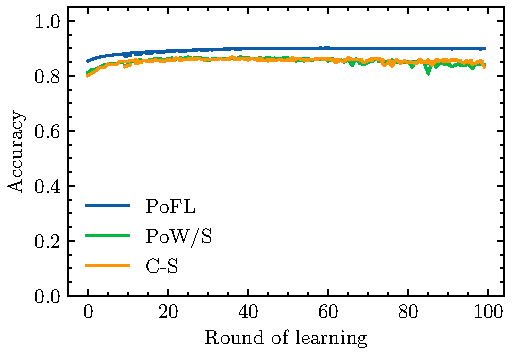
\includegraphics[width=\linewidth]{figuras/graficas/original_fashion_one.pdf}
  \caption{Fashion EMNIST (Tarea original).}
  %\label{fig:sfig3}
\end{subfigure} 
\begin{subfigure}{0.49\linewidth}
  \centering
  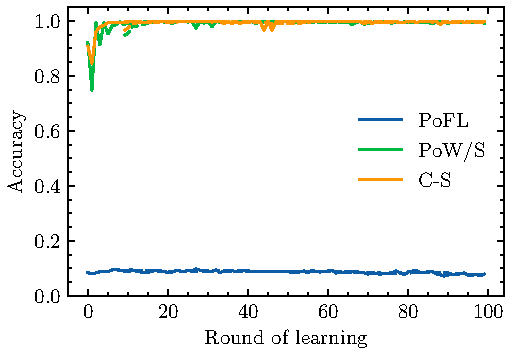
\includegraphics[width=\linewidth]{figuras/graficas/backdoor_fashion_one.pdf}
  \caption{Fashion EMNIST (Tarea backdoor).}
  %\label{fig:sfig2}
\end{subfigure}
\vskip\baselineskip
\begin{subfigure}{0.49\linewidth}
  \centering
  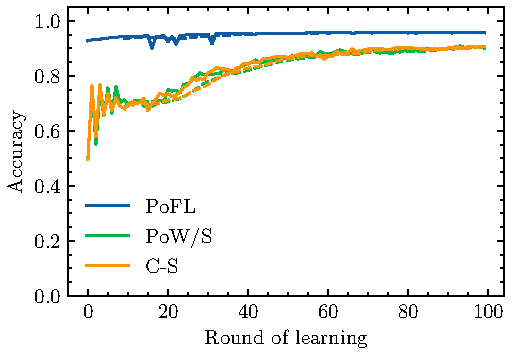
\includegraphics[width=\linewidth]{figuras/graficas/original_cifar_one.pdf}
  \caption{CIFAR (Tarea original).}
  %\label{fig:sfig2}
\end{subfigure}
\begin{subfigure}{0.49\linewidth}
  \centering
  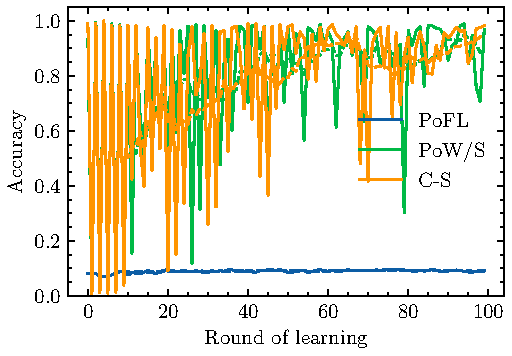
\includegraphics[width=\linewidth]{figuras/graficas/backdoor_cifar_one.pdf}
  \caption{CIFAR (Tarea backdoor).}
  %\label{fig:sfig4}
\end{subfigure}
\vskip\baselineskip
\caption{$accuracy$ (línea) y $accuracy_{10}$ (línea discontinua) de las tareas originales y backdoor en EMNIST (a y b), Fashion MNIST (c y d) y CIFAR (e y f), respectivamente, en el \textbf{escenario A}.}
\label{fig:pofl_a_backdoor}
\end{figure}

Basándonos en estas observaciones, los resultados experimentales ofrecen pruebas convincentes de que \ac{PoFL} constituye una arquitectura de \textit{blockchain} aplicada a \ac{FL} robusta contra ataques de \textit{backdoor} y bizantinos dentro del escenario investigado. Estos hallazgos confirman que el mecanismo de consenso basado en el rendimiento empleado por \textit{PoFL}, junto con la arquitectura de \textit{pooled-mining}, filtra de manera eficaz las actualizaciones maliciosas inyectadas por clientes adversarios debido a que estos tienden a crear actualizaciones con mala calidad.

\begin{table*}[!ht]
\centering
\begin{tabular}{lrrrrrr}
\toprule
 & \multicolumn{3}{c}{\textit{accuracy}} & \multicolumn{3}{c}{\textit{$accuracy_{10}$}}   \\
\toprule
       & \textbf{C-S} & \textbf{PoW/S} & \textbf{PoFL} & \textbf{C-S} & \textbf{PoW/S} & \textbf{PoFL}  \\ 
\toprule
\textbf{EMNIST} & 0.8931& 0.1000& \textbf{0.9926}& 0.6594& 0.1030& \textbf{0.9925}\\  
\midrule
\textbf{Fashion MNIST}& 0.8264& 0.1041& \textbf{0.9051}& 0.8363& 0.0978& \textbf{0.9049}\\ 
\midrule
\textbf{CIFAR-10}        & 0.2868& 0.6870& \textbf{0.9628}& 0.4196& 0.6685& \textbf{0.9604}\\
\bottomrule
\end{tabular}
\caption{\textit{accuracy} y \textit{$accuracy_{10}$} comparando PoFL con las arquitecturas de referencia en el \textbf{escenario A} ante un ataque bizantino.}\label{tab:poflbyzantine_a}

\end{table*}


\begin{figure}[!ht]
\begin{subfigure}{0.49\linewidth}
  \centering
  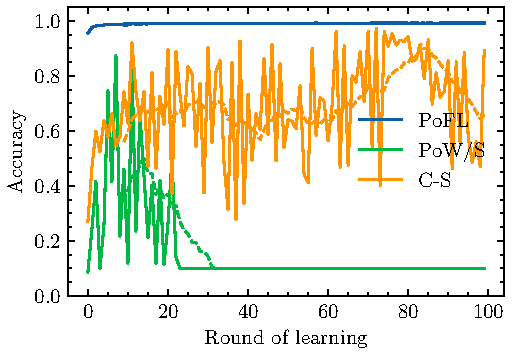
\includegraphics[width=\linewidth]{figuras/graficas/byzantine_mnist_one.pdf}
  \caption{EMNIST.}
  %\label{fig:sfig1}
\end{subfigure} 
\begin{subfigure}{0.49\linewidth}
  \centering
  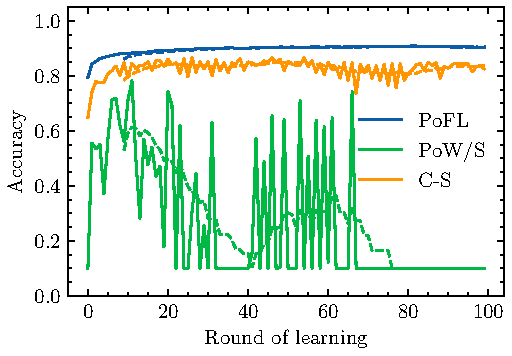
\includegraphics[width=\linewidth]{figuras/graficas/byzantine_fashion_one.pdf}
  \caption{Fashion EMNIST.}
  %\label{fig:sfig3}
\end{subfigure} 
\vskip\baselineskip
\centering
\begin{subfigure}{0.49\linewidth}
  \centering
  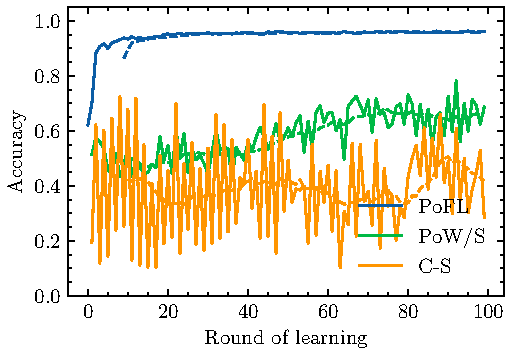
\includegraphics[width=\linewidth]{figuras/graficas/byzantine_cifar_one.pdf}
  \caption{CIFAR.}
  %\label{fig:sfig2}
\end{subfigure}
\vskip\baselineskip
\caption{$accuracy$ (línea) y $accuracy_{10}$ (línea discontinua) de las tareas originales  EMNIST (a), Fashion MNIST (b) y CIFAR (c), bajo un ataque bizantino en el \textbf{escenario A}.}
\label{fig:pofl_byzantine_a}
\end{figure}

\newpage
\subsection{Escenario B: Todos los mineros son atacados}\label{sec:pofl_b}
A continuación estudiamos el rendimiento de \ac{PoFL} como defensa en el \textbf{escenario B}. Los resultados han sido representados tanto en las Tablas \ref{tab:poflbackdoor_b} y \ref{tab:poflbyzantine_b} como en las Figuras \ref{fig:pofl_b_backdoor} y \ref{fig:pofl_byzantine_b}. Tras su observación llegamos a las siguientes conclusiones:
\begin{itemize}
	\item A diferencia del escenario anterior, donde \ac{PoFL} aparecía como la arquitectura con mayor rendimiento, en este caso exhibe el peor rendimiento en la mayoría de las tareas. En todas ellas muestra un comportamiento inconsistente con grandes fluctuaciones durante todo el proceso de entrenamiento. Nuestras arquitecturas de referencia, sin embargo, mantienen una precisión similar en todas las pruebas en comparación con el escenario anterior.
	
	\item En la tarea de \textit{backdoor}, acudiendo a la Tabla \ref{tab:poflbackdoor_b} y Figura \ref{fig:pofl_b_backdoor}, vemos como \ac{PoFL} tiene el peor rendimiento en la tarea original en los tres conjuntos. Además, aunque inferior a las arquitecturas de referencia, \ac{PoFL} muestra un alto rendimiento en la tarea secundaria indicando el éxito del ataque de \textit{backdoor} bajo estas circunstancias.
	
	\item Respecto al ataque bizantino, observando la Tabla \ref{tab:poflbyzantine_b} y Figura \ref{fig:pofl_byzantine_b}, vemos que el rendimiento de \ac{PoFL} es similar al de las arquitecturas de referencia, denotando ser vulnerable ante este tipo de ataques.
\end{itemize}


\begin{table}

    \centering
    \begin{tabular}{llcccccc}
    	\toprule
           &&\multicolumn{3}{c}{\textit{accuracy}}&  \multicolumn{3}{c}{\textit{$accuracy_{10}$}}\\
           \toprule
           &&\textbf{C-S} &  \textbf{PoW/S} &  \textbf{PoFL} &  \textbf{C-S} &  \textbf{PoW/S} & \textbf{PoFL} 
\\
\toprule
           \textbf{EMNIST} &Original 
&0.9863        &  \textbf{0.9889}  &  0.8986&  0.9866        &  0.9888  & \textbf{0.9108} 
\\
           &Backdoor 
&0.9999        &  1.0000     &  \textbf{0.7536}   &  0.9997        &  1.0000     & \textbf{0.8002} 
\\
\midrule
           \textbf{Fashion}   &Original 
&0.8593        &  \textbf{0.8729}  &  0.8133    &  0.9997        &  1.0000     & \textbf{0.8002} 
\\
           \textbf{MNIST}    &Backdoor 
&0.9955        &  0.9977  &  \textbf{0.8199} &  0.9891        &  0.9963  & \textbf{0.9181}
\\
\midrule
           \textbf{CIFAR-10}        &Original 
&0.9101        &  \textbf{0.9436}  &  0.8485  &  0.9032        &  \textbf{0.9402}  & 0.8223 
\\
           &Backdoor &0.9676        &  0.9922  &  \textbf{0.8535}   &  0.9837        &  0.9928  & \textbf{0.9151} \\
           \bottomrule
    \end{tabular}
    \caption{\textit{accuracy} y \textit{$accuracy_{10}$} comparando PoFL con las arquitecturas de referencia en el \textbf{escenario B} ante un ataque de backdoor.}\label{tab:poflbackdoor_b}
\end{table}


\begin{figure}[h!]
\begin{subfigure}{0.49\linewidth}
  \centering
  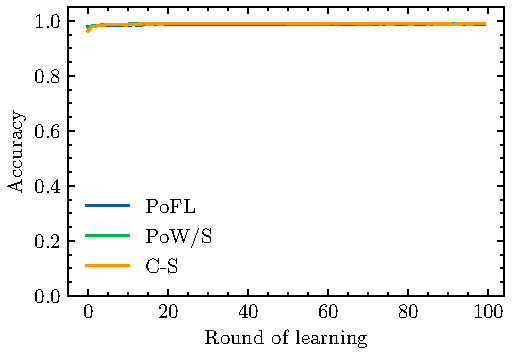
\includegraphics[width=\linewidth]{figuras/graficas/original_mnist_all.pdf}
  \caption{EMNIST (Tarea original).}
  %\label{fig:sfig1}
\end{subfigure} 
\begin{subfigure}{0.49\linewidth}
  \centering
  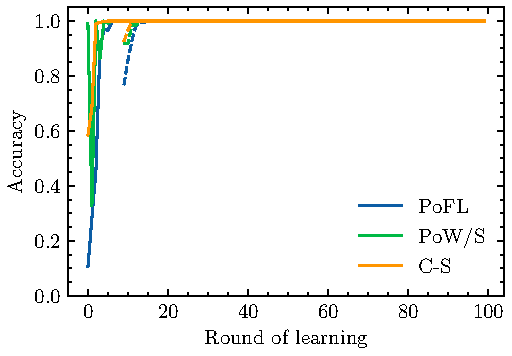
\includegraphics[width=\linewidth]{figuras/graficas/backdoor_mnist_all.pdf}
  \caption{EMNIST (Tarea backdoor).}
  %\label{fig:sfig1}
\end{subfigure} 
\vskip\baselineskip
\begin{subfigure}{0.49\linewidth}
  \centering
  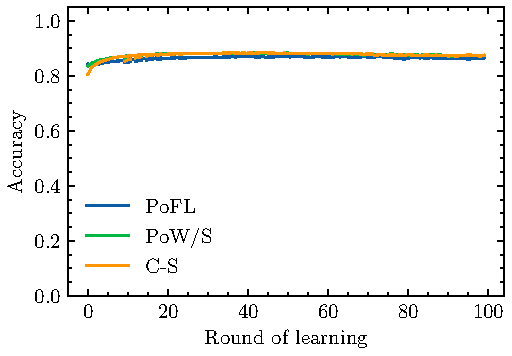
\includegraphics[width=\linewidth]{figuras/graficas/original_fashion_all.pdf}
  \caption{Fashion EMNIST (Tarea original).}
  %\label{fig:sfig3}
\end{subfigure} 
\begin{subfigure}{0.49\linewidth}
  \centering
  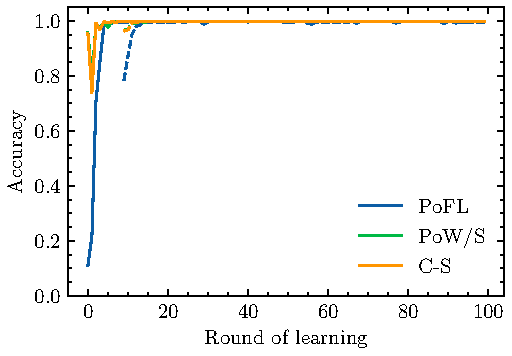
\includegraphics[width=\linewidth]{figuras/graficas/backdoor_fashion_all.pdf}
  \caption{Fashion EMNIST (Tarea backdoor).}
  %\label{fig:sfig2}
\end{subfigure}
\vskip\baselineskip
\begin{subfigure}{0.49\linewidth}
  \centering
  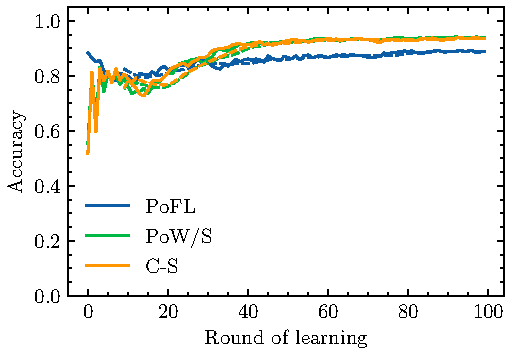
\includegraphics[width=\linewidth]{figuras/graficas/original_cifar_all.pdf}
  \caption{CIFAR (Tarea original).}
  %\label{fig:sfig2}
\end{subfigure}
\begin{subfigure}{0.49\linewidth}
  \centering
  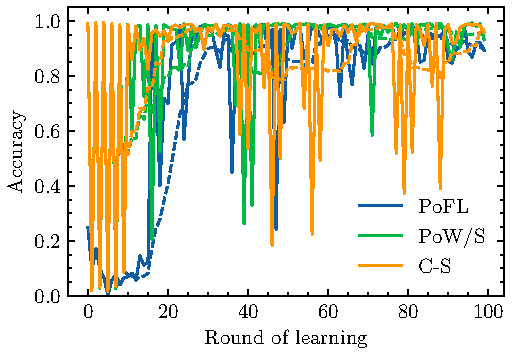
\includegraphics[width=\linewidth]{figuras/graficas/backdoor_cifar_all.pdf}
  \caption{CIFAR (Tarea backdoor).}
  %\label{fig:sfig4}
\end{subfigure}
\vskip\baselineskip
\caption{$accuracy$ (línea) y $accuracy_{10}$ (línea discontinua) de las tareas originales y backdoor en EMNIST (a y b), Fashion MNIST (c y d) y CIFAR (e y f), respectivamente, en el \textbf{escenario B}.}
\label{fig:pofl_b_backdoor}
\end{figure}
\begin{table}
    \centering
    \begin{tabular}{lcccccc}
    	\toprule
           &\multicolumn{3}{c}{\textit{accuracy}}&  \multicolumn{3}{c}{\textit{$accuracy_{10}$}}\\
           \toprule
           &\textbf{C-S} &  \textbf{PoW/S} &  \textbf{PoFL} &  \textbf{C-S} &  \textbf{PoW/S} & \textbf{PoFL} 
\\
\toprule
           \textbf{EMNIST} &\textbf{0.9232}&  0.7351&  0.9202&  0.7770&  0.7246& \textbf{0.9120}\\
           \midrule
           \textbf{Fashion MNIST}&\textbf{0.8329}&  0.7372&  0.7344&  \textbf{0.8222}&  0.8087& 0.7476\\
           \midrule
           \textbf{CIFAR-10}        &0.6168&  \textbf{0.7967}&  0.5648&  0.6692&  \textbf{0.7545}& 0.5648\\
           \bottomrule
    \end{tabular}
    \caption{\textit{accuracy} y \textit{$accuracy_{10}$} comparando PoFL con las arquitecturas de referencia en el \textbf{escenario B} ante un ataque de bizantino.}\label{tab:poflbyzantine_b}

\end{table}
\begin{figure}[!ht]
\begin{subfigure}{0.49\linewidth}
  \centering
  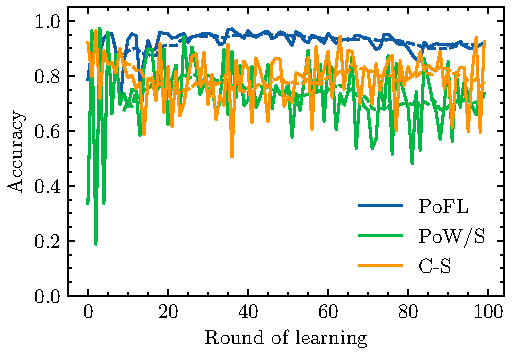
\includegraphics[width=\linewidth]{figuras/graficas/byzantine_mnist_all.pdf}
  \caption{EMNIST.}
  %\label{fig:sfig1}
\end{subfigure} 
\begin{subfigure}{0.49\linewidth}
  \centering
  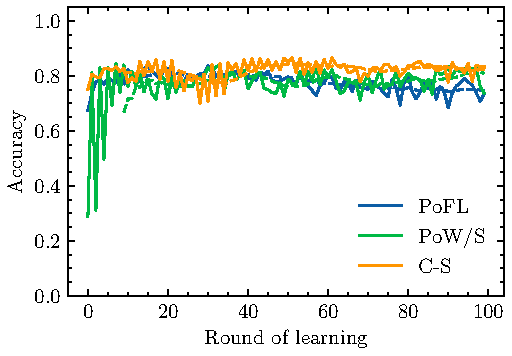
\includegraphics[width=\linewidth]{figuras/graficas/byzantine_fashion_all.pdf}
  \caption{Fashion EMNIST.}
  %\label{fig:sfig3}
\end{subfigure} 
\vskip\baselineskip
\centering
\begin{subfigure}{0.49\linewidth}
  \centering
  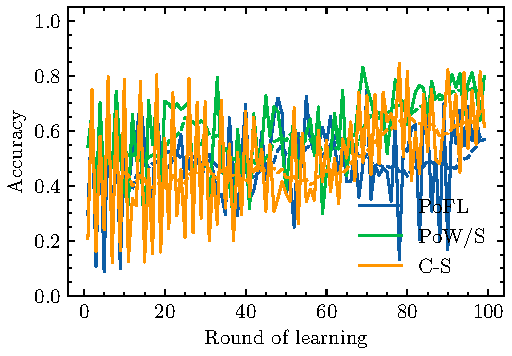
\includegraphics[width=\linewidth]{figuras/graficas/byzantine_cifar_all.pdf}
  \caption{CIFAR.}
  %\label{fig:sfig2}
\end{subfigure}
\vskip\baselineskip
\caption{$accuracy$ (línea) y $accuracy_{10}$ (línea discontinua) de las tareas originales  EMNIST (a), Fashion MNIST (b) y CIFAR (c), bajo un ataque bizantino en el \textbf{escenario B}.}
\label{fig:pofl_byzantine_b}
\end{figure}

En conclusión, los experimentos muestran un panorama preocupante sobre la idoneidad de \ac{PoFL} en este escenario. Como se ha demostrado en las observaciones anteriores, \ac{PoFL} exhibe una vulnerabilidad significativa a los ataques de \textit{backdoor}. No solo logra una precisión preocupantemente alta en las tareas de \textit{backdoor} en promedio, sino que su rendimiento en la tarea original también sufre un detrimento sustancial. Además, muestra un deterioro grave ante ataques bizantinos, obteniendo resultados similares a aquellos obtenidos por nuestras arquitecturas de referencia. Esto se debe a que cuando el rendimiento de todas las \textit{pools} se ve comprometido, el mecanismo de consenso es incapaz de filtrar las actualizaciones maliciosas.

Esta vulnerabilidad de \ac{PoFL} motiva el diseño de \ac{KFC}, como la combinación de \ac{PoFL} y un mecanismo de defensa en cada minero, lo que lo hace resistente a ataques adversarios incluso cuando todos los mineros están siendo atacados. Abordamos esta cuestión en la siguiente sección.


\newpage
\section{Análisis de rendimiento de KFC}\label{sec:kfc_experiments}
En esta sección analizaremos los resultados de \ac{KFC} en los escenarios A (vea Sección \ref{sec:kfc_a}) y B (vea Sección \ref{sec:kfc_b}). Además, los compararemos con aquellos de \ac{PoFL} obtenidos en la Sección \ref{sec:hipotesis}.

\subsection{Escenario A: Un solo atacante}\label{sec:kfc_a}

Primero nos centraremos en el \textbf{escenario A} donde \ac{PoFL} ya se mostraba como una defensa válida. Los resultados expuestos en las Tablas \ref{tab:kfcbackdoor_a} y \ref{tab:kfcbyzantine_a} junto a las Figuras \ref{fig:kfc_a} y \ref{fig:kfc_byzantine_a}, nos indican que \ac{KFC} también es una defensa eficaz para ambos tipos de ataques. Si observamos con detalle, vemos que el rendimiento de \ac{KFC} tanto en la tarea original del ataque de \textit{backdoor} como en el ataque bizantino es ligeramente inferior al de \ac{PoFL}. Esto es un resultado esperado y conocido del mecanismo de agregación Krum~\cite{krum-2017}, debido a seleccionar únicamente al cliente que minimiza la distancia geométrica, lo que causa una pérdida de precisión en la tarea original pero también en la tarea de \textit{backdoor}. Podemos concluir por tanto que \ac{KFC} se presenta en este escenario como una arquitectura viable para implementar \ac{FL} y \textit{blockchain} mientras ofrece una capa de seguridad, siendo igual de viable que \ac{PoFL} pues ambas tienen sus características.


\begin{table*}[h!]
\centering
\begin{tabular}{llrrrr}
\toprule
 & & \multicolumn{2}{c}{\textit{accuracy}} & \multicolumn{2}{c}{\textit{$accuracy_{10}$}}   \\
 \toprule
\textbf{}     &          & \textbf{PoFL}    & \textbf{KFC} & \textbf{PoFL}    & \textbf{KFC} \\ 
\midrule
\textbf{EMNIST}        & Original &   \textbf{0.9930}&  0.9889& \textbf{0.9930}& 0.9887 \\ 
              & Backdoor &     0.0980& \textbf{0.0964}&    0.0979&     \textbf{ 0.0970} \\ 
\midrule
\textbf{Fashion} & Original &    \textbf{0.8961}& 0.8645&  \textbf{0.8986}&   0.8645    \\ 
\textbf{MNIST}  & Backdoor &   0.0871& \textbf{0.0768}&  0.0989   &  \textbf{0.0813}    \\ 
\midrule
\textbf{CIFAR-10}      & Original & \textbf{0.9397}& 0.8870& \textbf{0.9283}& 0.8839\\ 
                        & Backdoor &  0.1163& \textbf{0.1025}& \textbf{0.0849}&  0.0981\\ 
\bottomrule
\end{tabular}
    \caption{\textit{accuracy} y \textit{$accuracy_{10}$} comparando PoFL y KFC en el \textbf{escenario A} ante un ataque de backdoor.} \label{tab:kfcbackdoor_a}

\end{table*}


\begin{figure}[h!]
\begin{subfigure}{0.49\linewidth}
  \centering
  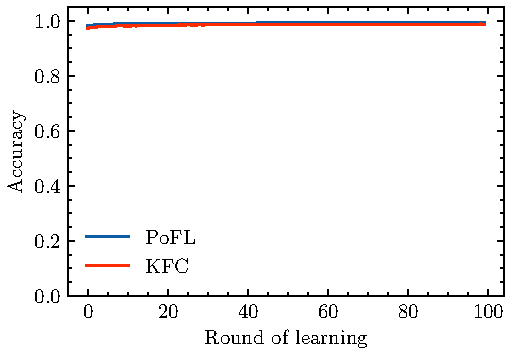
\includegraphics[width=\linewidth]{figuras/graficas/kfc_vs_pofl_original_mnist_one.pdf}
  \caption{EMNIST (Tarea original).}
  %\label{fig:sfig1}
\end{subfigure} 
\begin{subfigure}{0.49\linewidth}
  \centering
  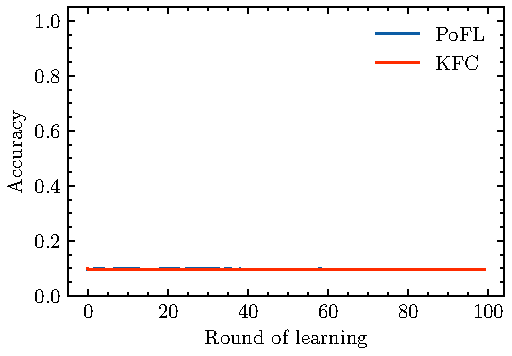
\includegraphics[width=\linewidth]{figuras/graficas/kfc_vs_pofl_backdoor_mnist_one.pdf}
  \caption{EMNIST (Tarea backdoor).}
  %\label{fig:sfig1}
\end{subfigure} 
\vskip\baselineskip
\begin{subfigure}{0.49\linewidth}
  \centering
  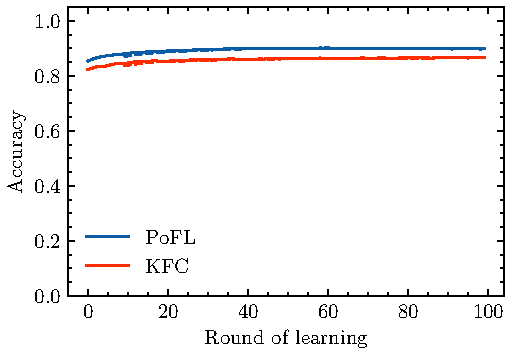
\includegraphics[width=\linewidth]{figuras/graficas/kfc_vs_pofl_original_fashion_one.pdf}
  \caption{Fashion EMNIST (Tarea original).}
  %\label{fig:sfig3}
\end{subfigure} 
\begin{subfigure}{0.49\linewidth}
  \centering
  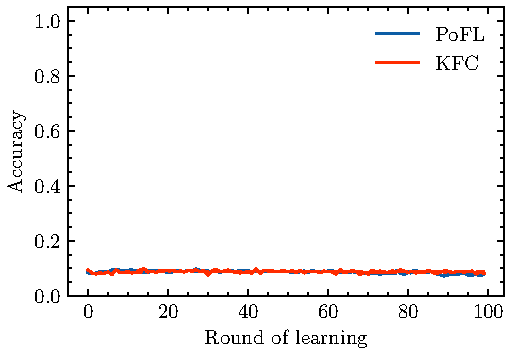
\includegraphics[width=\linewidth]{figuras/graficas/kfc_vs_pofl_backdoor_fashion_one.pdf}
  \caption{Fashion EMNIST (Tarea backdoor).}
  %\label{fig:sfig2}
\end{subfigure}
\vskip\baselineskip
\begin{subfigure}{0.49\linewidth}
  \centering
  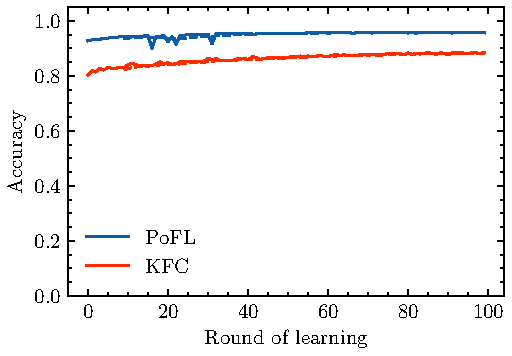
\includegraphics[width=\linewidth]{figuras/graficas/kfc_vs_pofl_original_cifar_one.pdf}
  \caption{CIFAR (Tarea original).}
  %\label{fig:sfig2}
\end{subfigure}
\begin{subfigure}{0.49\linewidth}
  \centering
  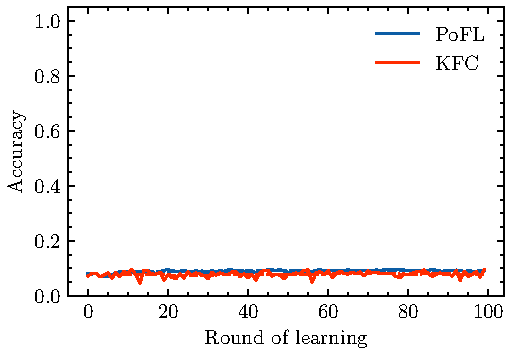
\includegraphics[width=\linewidth]{figuras/graficas/kfc_vs_pofl_backdoor_cifar_one.pdf}
  \caption{CIFAR (Tarea backdoor).}
  %\label{fig:sfig4}
\end{subfigure}
\vskip\baselineskip
\caption{$accuracy$ (linea) y $accuracy_{10}$ (linea discontinua) de la tarea original y backdoor en EMNIST (a y b), Fashion MNIST (c y d) y CIFAR (e y f), respectivamente, en el \textbf{escenario A}.}
\label{fig:kfc_a}
\end{figure}


\begin{table*}[h!]
\centering
\begin{tabular}{lrrrr}
\toprule
 & \multicolumn{2}{c}{\textit{accuracy}} & \multicolumn{2}{c}{\textit{$accuracy_{10}$}}   \\
 \toprule
\textbf{}     & \textbf{PoFL}    & \textbf{KFC} & \textbf{PoFL}    & \textbf{KFC} \\ 
\midrule
\textbf{EMNIST}        &   \textbf{0.9926}&  0.9882& \textbf{0.9925}& 0.9880\\ 
\midrule
\textbf{Fashion MNIST}&    \textbf{0.9051}& 0.8705&  \textbf{0.9049}&   0.8684\\ 
\midrule
\textbf{CIFAR-10}      & \textbf{0.9628}& 0.8901& \textbf{0.9604}& 0.8875\\
\bottomrule
\end{tabular}
    \caption{\textit{accuracy} y \textit{$accuracy_{10}$} comparando PoFL y KFC en el \textbf{escenario A} ante un ataque bizantino.}  \label{tab:kfcbyzantine_a}

\end{table*}


\begin{figure}[!ht]
\begin{subfigure}{0.49\linewidth}
  \centering
  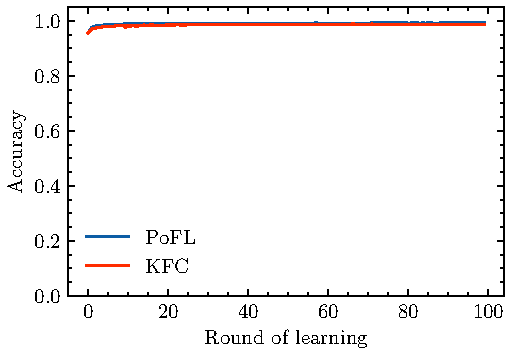
\includegraphics[width=\linewidth]{figuras/graficas/kfc_vs_pofl_byzantine_mnist_one.pdf}
  \caption{EMNIST.}
  %\label{fig:sfig1}
\end{subfigure} 
\begin{subfigure}{0.49\linewidth}
  \centering
  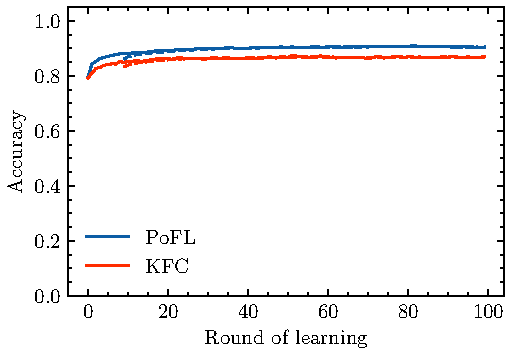
\includegraphics[width=\linewidth]{figuras/graficas/kfc_vs_pofl_byzantine_fashion_one.pdf}
  \caption{Fashion EMNIST.}
  %\label{fig:sfig3}
\end{subfigure} 
\vskip\baselineskip
\centering
\begin{subfigure}{0.49\linewidth}
  \centering
  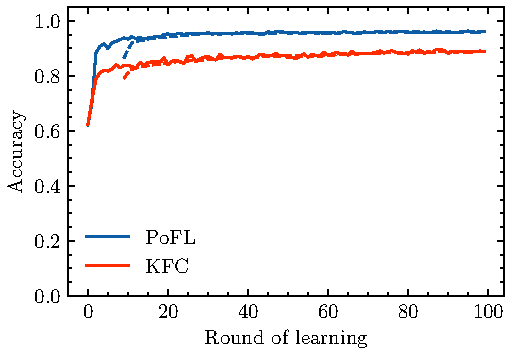
\includegraphics[width=\linewidth]{figuras/graficas/kfc_vs_pofl_byzantine_cifar_one.pdf}
  \caption{CIFAR.}
  %\label{fig:sfig2}
\end{subfigure}
\vskip\baselineskip
\caption{$accuracy$ (línea) y $accuracy_{10}$ (línea discontinua) de las tareas originales  EMNIST (a), Fashion MNIST (b) y CIFAR (c), bajo un ataque bizantino en el \textbf{escenario A}.}
\label{fig:kfc_byzantine_a}
\end{figure}


\subsection{Escenario B: Todos los mineros son atacados}\label{sec:kfc_b}

En esta sección volvemos al escenario más exigente en el que ya no se puede asumir la existencia de una \textit{pool} no siendo atacada. Los resultados de \ac{KFC} en este escenario se muestran en las Tablas \ref{tab:kfcbackdoorb} y \ref{tab:kfcbyzantine_b} y Figuras \ref{fig:kfc_b_backdoor} y \ref{fig:kfc_byzantine_b}. Un análisis detallado de los resultados nos lleva a las siguientes conclusiones comunes:

\begin{itemize}
	\item La capacidad de \ac{KFC} para mantener la precisión en la tarea original de \textit{backdoor} en comparación con \ac{PoFL} demuestra su resistencia en el nuevo escenario donde todos los mineros están bajo ataque.
    \item Al el contrario que \ac{PoFL}, \ac{KFC} demuestra una resistencia excepcional ante todos los ataques, logrando una precisión mínima en la tarea de \textit{backdoor} y mantener el rendimiento en el ataque bizantino, mitigando efectivamente los ataques.
\end{itemize}

En resumen, \ac{KFC} destaca como mecanismo de defensa. Los resultados nos indica como logra mitigar ambos tipos de ataques considerados, logrando reducir el impacto de la \textit{backdoor} mientras se observa un rendimiento alto en la tarea original y en el ataque de tipo bizantino, superando a \ac{PoFL} y nuestras arquitecturas de referencia en los entornos de la experimentación. Estos hallazgos confirman con firmeza que \ac{KFC} supera a \ac{PoFL} como la mejor opción en escenarios donde todas las \textit{pools} podrían estar comprometidas. \ac{KFC} logra eficazmente el doble objetivo de defender contra los ataques de \textit{backdoor} en \ac{FL}: maximizar el rendimiento de la tarea original y minimizar el impacto de la tarea inyectada. Además, su rendimiento contra ataques bizantinos se muestra excelente al presentar un comportamiento estable y una alta precisión. Esto se debe a que el mecanismo de agregación Krum permite filtrar actualizaciones maliciosas dentro de cada \textit{pool} y logrando así que el mecanismo de consenso basado en rendimiento ofrezca un modelo no comprometido.



\begin{table}
    \centering
    \begin{tabular}{llcccc}
    	\toprule
            &&\multicolumn{2}{c}{\textit{accuracy}}&  \multicolumn{2}{c}{\textit{$accuracy_{10}$}
}\\
\toprule
            &&\textbf{PoFL}    &  \textbf{KFC} &  & \textbf{KFC}
\\
\toprule
            \textbf{EMNIST}        &Original 
&0.8986  &  \textbf{0.9921}  &  0.9108 & \textbf{0.9922}    
\\
            &Backdoor 
&0.7536  &  \textbf{0.0995}   &  0.8002 & \textbf{0.0994}     
\\
\midrule
            \textbf{Fashion} &Original 
&0.8133 &  \textbf{0.9000}   &  0.8002 & \textbf{0.9000}    
\\
            \textbf{MNIST}  &Backdoor 
&0.8199  &  \textbf{0.0958}  &  0.9181 & \textbf{0.0894}    
\\
\midrule
            \textbf{CIFAR-10}      &Original 
&\textbf{0.8485}  &  0.8214  &  0.8223 & \textbf{0.9123}     
\\
            &Backdoor &0.8535  &  \textbf{0.1163}  &  0.9151 & \textbf{0.1016}    \\
\bottomrule
    \end{tabular}
     \caption{\textit{accuracy} y \textit{$accuracy_{10}$} comparando PoFL y KFC en el \textbf{escenario B} ante un ataque de backdoor.}
    \label{tab:kfcbackdoorb}
\end{table}

\begin{figure}[h!]
\begin{subfigure}{0.49\linewidth}
  \centering
  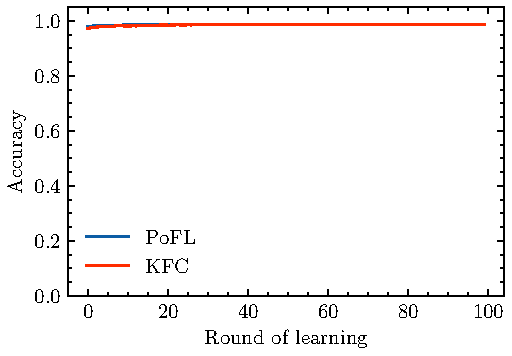
\includegraphics[width=\linewidth]{figuras/graficas/pofl_vs_kfc_original_mnist_all.pdf}
  \caption{EMNIST (Tarea original).}
  %\label{fig:sfig1}
\end{subfigure} 
\begin{subfigure}{0.49\linewidth}
  \centering
  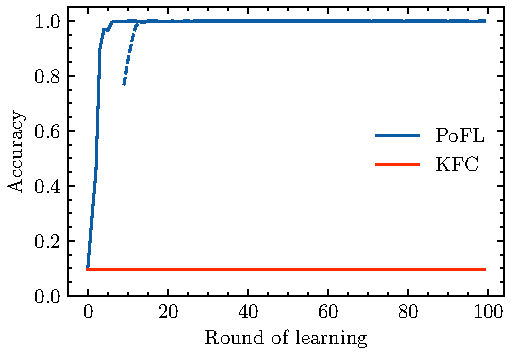
\includegraphics[width=\linewidth]{figuras/graficas/pofl_vs_kfc_backdoor_mnist_all.pdf}
  \caption{EMNIST (Tarea backdoor).}
  %\label{fig:sfig1}
\end{subfigure} 
\vskip\baselineskip
\begin{subfigure}{0.49\linewidth}
  \centering
  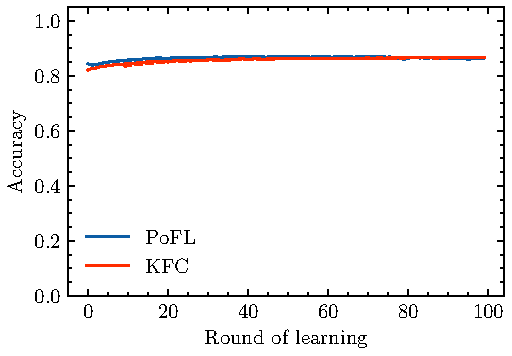
\includegraphics[width=\linewidth]{figuras/graficas/pofl_vs_kfc_original_fashion_all.pdf}
  \caption{Fashion EMNIST (Tarea original).}
  %\label{fig:sfig3}
\end{subfigure} 
\begin{subfigure}{0.49\linewidth}
  \centering
  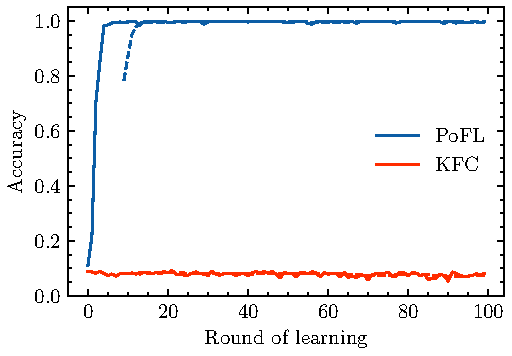
\includegraphics[width=\linewidth]{figuras/graficas/pofl_vs_kfc_backdoor_fashion_all.pdf}
  \caption{Fashion EMNIST (Tarea backdoor).}
  %\label{fig:sfig2}
\end{subfigure}
\vskip\baselineskip
\begin{subfigure}{0.49\linewidth}
  \centering
  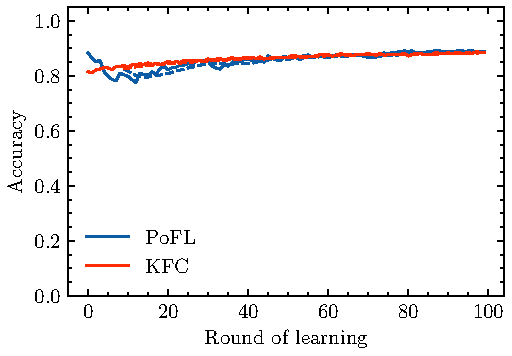
\includegraphics[width=\linewidth]{figuras/graficas/pofl_vs_kfc_original_cifar_all.pdf}
  \caption{CIFAR (Tarea original).}
  %\label{fig:sfig2}
\end{subfigure}
\begin{subfigure}{0.49\linewidth}
  \centering
  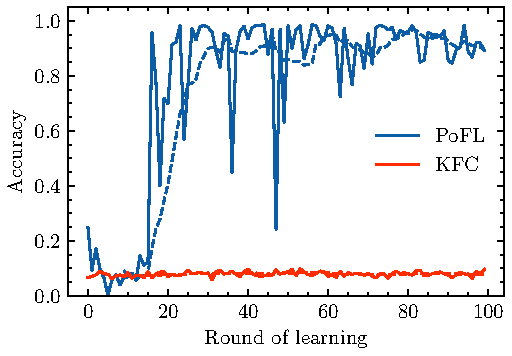
\includegraphics[width=\linewidth]{figuras/graficas/pofl_vs_kfc_backdoor_cifar_all.pdf}
  \caption{CIFAR (Tarea backdoor).}
  %\label{fig:sfig4}
\end{subfigure}
\vskip\baselineskip
\caption{$accuracy$ (linea) y $accuracy_{10}$ (linea discontinua) de la tarea original y backdoor en EMNIST (a y b), Fashion MNIST (c y d) y CIFAR (e y f), respectivamente, en el \textbf{escenario B}.}
\label{fig:kfc_b_backdoor}
\end{figure}

\begin{table*}[h!]
\centering
\begin{tabular}{lrrrr}
\toprule
 & \multicolumn{2}{c}{\textit{accuracy}} & \multicolumn{2}{c}{\textit{$accuracy_{10}$}}   \\
 \toprule
\textbf{}     & \textbf{PoFL}    & \textbf{KFC} & \textbf{PoFL}    & \textbf{KFC} \\ 
\midrule
\textbf{EMNIST}        &   0.9202&  \textbf{0.9881}& 0.9120& \textbf{0.9881}\\ 
\midrule
\textbf{Fashion MNIST}&    0.7344& \textbf{0.8709}&  0.7476&   \textbf{0.8690}\\ 
\midrule
\textbf{CIFAR-10}      & 0.5681& \textbf{0.8856}& 0.5648& \textbf{0.8914}\\
\bottomrule
\end{tabular}
    \caption{\textit{accuracy} y \textit{$accuracy_{10}$} comparando PoFL y KFC en el \textbf{escenario B} ante un ataque bizantino.}  \label{tab:kfcbyzantine_b}

\end{table*}


\begin{figure}[!ht]
\begin{subfigure}{0.49\linewidth}
  \centering
  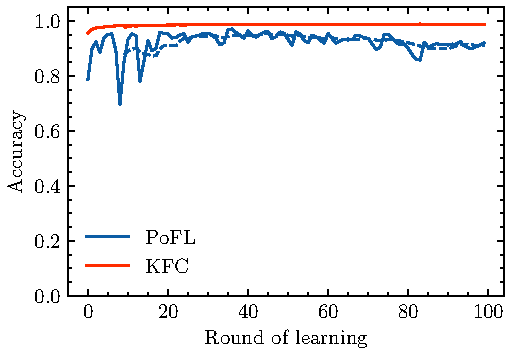
\includegraphics[width=\linewidth]{figuras/graficas/pofl_vs_kfc_byzantine_mnist_all.pdf}
  \caption{EMNIST.}
  %\label{fig:sfig1}
\end{subfigure} 
\begin{subfigure}{0.49\linewidth}
  \centering
  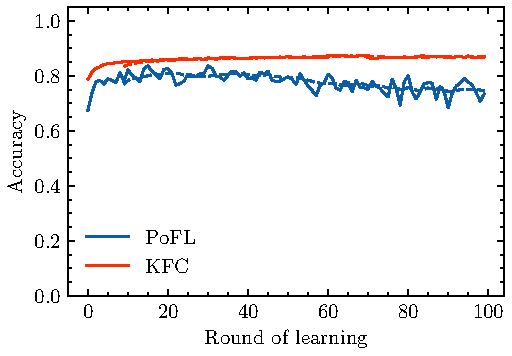
\includegraphics[width=\linewidth]{figuras/graficas/pofl_vs_kfc_byzantine_fashion_all.pdf}
  \caption{Fashion EMNIST.}
  %\label{fig:sfig3}
\end{subfigure} 
\vskip\baselineskip
\centering
\begin{subfigure}{0.49\linewidth}
  \centering
  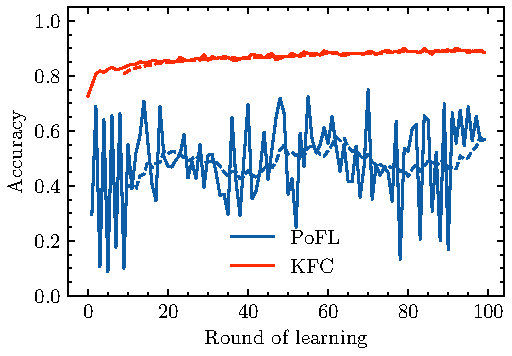
\includegraphics[width=\linewidth]{figuras/graficas/pofl_vs_kfc_byzantine_cifar_all.pdf}
  \caption{CIFAR.}
  %\label{fig:sfig2}
\end{subfigure}
\vskip\baselineskip
\caption{$accuracy$ (línea) y $accuracy_{10}$ (línea discontinua) de las tareas originales  EMNIST (a), Fashion MNIST (b) y CIFAR (c), bajo un ataque bizantino en el \textbf{escenario B}.}
\label{fig:kfc_byzantine_b}
\end{figure}